\chapter{My Research Overview} 
\label{chapter-my-research} 



\tikzset{every picture/.style={line width=0.75pt}} %set default line width to 0.75pt        

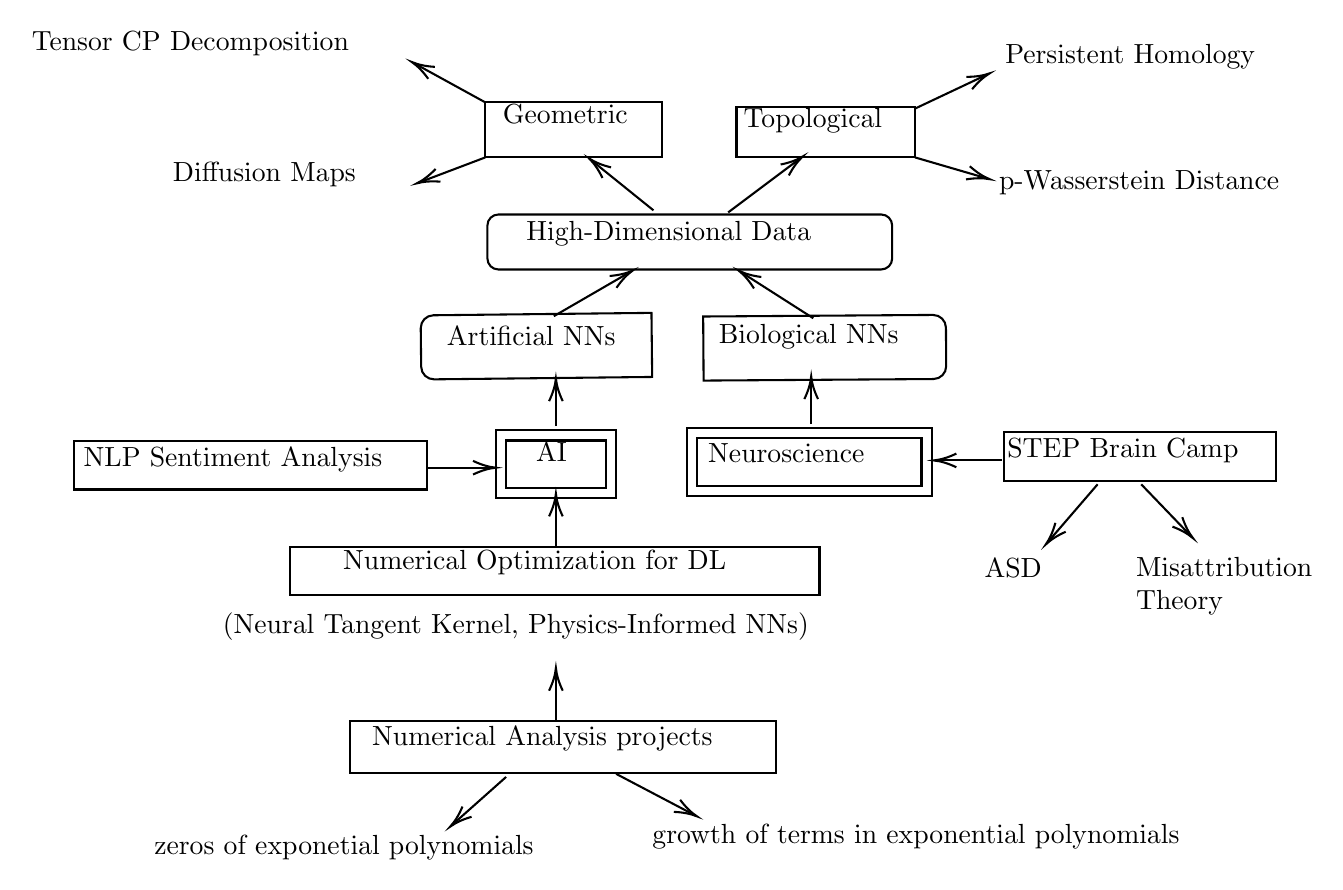
\begin{tikzpicture}[x=0.75pt,y=0.75pt,yscale=-1,xscale=1]
%uncomment if require: \path (0,570); %set diagram left start at 0, and has height of 570

%Shape: Rectangle [id:dp06677686134312855] 
\draw   (245,42.5) -- (330,42.5) -- (330,69) -- (245,69) -- cycle ;
%Straight Lines [id:da13012305376230948] 
\draw    (279,256.5) -- (279,233) ;
\draw [shift={(279,231)}, rotate = 90] [color={rgb, 255:red, 0; green, 0; blue, 0 }  ][line width=0.75]    (10.93,-3.29) .. controls (6.95,-1.4) and (3.31,-0.3) .. (0,0) .. controls (3.31,0.3) and (6.95,1.4) .. (10.93,3.29)   ;
%Rounded Same Side Corner Rect [id:dp1538787400275181] 
\draw   (220.32,175.93) .. controls (216.91,175.97) and (214.12,173.24) .. (214.08,169.83) -- (213.88,151.3) .. controls (213.84,147.89) and (216.57,145.1) .. (219.98,145.06) -- (325.04,143.91) .. controls (325.04,143.91) and (325.04,143.91) .. (325.04,143.91) -- (325.38,174.78) .. controls (325.38,174.78) and (325.38,174.78) .. (325.38,174.78) -- cycle ;
%Straight Lines [id:da5293910669002766] 
\draw    (279,198.5) -- (279,177.5) ;
\draw [shift={(279,175.5)}, rotate = 90] [color={rgb, 255:red, 0; green, 0; blue, 0 }  ][line width=0.75]    (10.93,-3.29) .. controls (6.95,-1.4) and (3.31,-0.3) .. (0,0) .. controls (3.31,0.3) and (6.95,1.4) .. (10.93,3.29)   ;
%Rounded Rect [id:dp6442511498883838] 
\draw   (246,101.8) .. controls (246,98.87) and (248.37,96.5) .. (251.3,96.5) -- (435.7,96.5) .. controls (438.63,96.5) and (441,98.87) .. (441,101.8) -- (441,117.7) .. controls (441,120.63) and (438.63,123) .. (435.7,123) -- (251.3,123) .. controls (248.37,123) and (246,120.63) .. (246,117.7) -- cycle ;
%Straight Lines [id:da6806416651326912] 
\draw    (278,145.5) -- (314.27,124.5) ;
\draw [shift={(316,123.5)}, rotate = 149.93] [color={rgb, 255:red, 0; green, 0; blue, 0 }  ][line width=0.75]    (10.93,-3.29) .. controls (6.95,-1.4) and (3.31,-0.3) .. (0,0) .. controls (3.31,0.3) and (6.95,1.4) .. (10.93,3.29)   ;
%Straight Lines [id:da617693416732219] 
\draw    (403,146.5) -- (368.69,124.58) ;
\draw [shift={(367,123.5)}, rotate = 32.57] [color={rgb, 255:red, 0; green, 0; blue, 0 }  ][line width=0.75]    (10.93,-3.29) .. controls (6.95,-1.4) and (3.31,-0.3) .. (0,0) .. controls (3.31,0.3) and (6.95,1.4) .. (10.93,3.29)   ;
%Straight Lines [id:da6384786986467668] 
\draw    (326,94.5) -- (296.56,70.76) ;
\draw [shift={(295,69.5)}, rotate = 38.88] [color={rgb, 255:red, 0; green, 0; blue, 0 }  ][line width=0.75]    (10.93,-3.29) .. controls (6.95,-1.4) and (3.31,-0.3) .. (0,0) .. controls (3.31,0.3) and (6.95,1.4) .. (10.93,3.29)   ;
%Straight Lines [id:da29416529890771037] 
\draw    (362,95.5) -- (396.4,69.7) ;
\draw [shift={(398,68.5)}, rotate = 143.13] [color={rgb, 255:red, 0; green, 0; blue, 0 }  ][line width=0.75]    (10.93,-3.29) .. controls (6.95,-1.4) and (3.31,-0.3) .. (0,0) .. controls (3.31,0.3) and (6.95,1.4) .. (10.93,3.29)   ;
%Shape: Frame [id:dp5175795866418891] 
\draw   (250,200.5) -- (308,200.5) -- (308,233) -- (250,233) -- cycle(303.13,205.38) -- (254.88,205.38) -- (254.88,228.13) -- (303.13,228.13) -- cycle ;
%Shape: Rectangle [id:dp33761076394518486] 
\draw   (366,44.5) -- (452,44.5) -- (452,69) -- (366,69) -- cycle ;
%Straight Lines [id:da6824079386581208] 
\draw    (402,197.5) -- (402,176.5) ;
\draw [shift={(402,174.5)}, rotate = 90] [color={rgb, 255:red, 0; green, 0; blue, 0 }  ][line width=0.75]    (10.93,-3.29) .. controls (6.95,-1.4) and (3.31,-0.3) .. (0,0) .. controls (3.31,0.3) and (6.95,1.4) .. (10.93,3.29)   ;
%Shape: Frame [id:dp6654281736387082] 
\draw   (342,199.5) -- (460,199.5) -- (460,232) -- (342,232) -- cycle(455.13,204.38) -- (346.88,204.38) -- (346.88,227.13) -- (455.13,227.13) -- cycle ;
%Shape: Rectangle [id:dp919524157463598] 
\draw   (495,201.5) -- (626,201.5) -- (626,225) -- (495,225) -- cycle ;
%Straight Lines [id:da3817096751621891] 
\draw    (245,42.5) -- (211.25,23.96) ;
\draw [shift={(209.5,23)}, rotate = 28.78] [color={rgb, 255:red, 0; green, 0; blue, 0 }  ][line width=0.75]    (10.93,-3.29) .. controls (6.95,-1.4) and (3.31,-0.3) .. (0,0) .. controls (3.31,0.3) and (6.95,1.4) .. (10.93,3.29)   ;
%Straight Lines [id:da5951890180419199] 
\draw    (245,69) -- (213.87,80.79) ;
\draw [shift={(212,81.5)}, rotate = 339.25] [color={rgb, 255:red, 0; green, 0; blue, 0 }  ][line width=0.75]    (10.93,-3.29) .. controls (6.95,-1.4) and (3.31,-0.3) .. (0,0) .. controls (3.31,0.3) and (6.95,1.4) .. (10.93,3.29)   ;
%Straight Lines [id:da19945747898475918] 
\draw    (452,45.5) -- (486.19,29.35) ;
\draw [shift={(488,28.5)}, rotate = 154.72] [color={rgb, 255:red, 0; green, 0; blue, 0 }  ][line width=0.75]    (10.93,-3.29) .. controls (6.95,-1.4) and (3.31,-0.3) .. (0,0) .. controls (3.31,0.3) and (6.95,1.4) .. (10.93,3.29)   ;
%Straight Lines [id:da8863365534257026] 
\draw    (452,69) -- (486.08,78.94) ;
\draw [shift={(488,79.5)}, rotate = 196.26] [color={rgb, 255:red, 0; green, 0; blue, 0 }  ][line width=0.75]    (10.93,-3.29) .. controls (6.95,-1.4) and (3.31,-0.3) .. (0,0) .. controls (3.31,0.3) and (6.95,1.4) .. (10.93,3.29)   ;
%Shape: Rectangle [id:dp1530626748145647] 
\draw   (47,205.5) -- (217,205.5) -- (217,229) -- (47,229) -- cycle ;
%Straight Lines [id:da6093367532546459] 
\draw    (217,218.5) -- (248,218.5) ;
\draw [shift={(250,218.5)}, rotate = 180] [color={rgb, 255:red, 0; green, 0; blue, 0 }  ][line width=0.75]    (10.93,-3.29) .. controls (6.95,-1.4) and (3.31,-0.3) .. (0,0) .. controls (3.31,0.3) and (6.95,1.4) .. (10.93,3.29)   ;
%Straight Lines [id:da8953994577866498] 
\draw    (494,215) -- (463,215) ;
\draw [shift={(461,215)}, rotate = 360] [color={rgb, 255:red, 0; green, 0; blue, 0 }  ][line width=0.75]    (10.93,-3.29) .. controls (6.95,-1.4) and (3.31,-0.3) .. (0,0) .. controls (3.31,0.3) and (6.95,1.4) .. (10.93,3.29)   ;
%Straight Lines [id:da2358792275861883] 
\draw    (540,226.5) -- (516.31,253.99) ;
\draw [shift={(515,255.5)}, rotate = 310.76] [color={rgb, 255:red, 0; green, 0; blue, 0 }  ][line width=0.75]    (10.93,-3.29) .. controls (6.95,-1.4) and (3.31,-0.3) .. (0,0) .. controls (3.31,0.3) and (6.95,1.4) .. (10.93,3.29)   ;
%Straight Lines [id:da8757816120359687] 
\draw    (561,226.5) -- (584.61,251.06) ;
\draw [shift={(586,252.5)}, rotate = 226.12] [color={rgb, 255:red, 0; green, 0; blue, 0 }  ][line width=0.75]    (10.93,-3.29) .. controls (6.95,-1.4) and (3.31,-0.3) .. (0,0) .. controls (3.31,0.3) and (6.95,1.4) .. (10.93,3.29)   ;
%Shape: Rectangle [id:dp7812645925768504] 
\draw   (151,256.5) -- (406,256.5) -- (406,280) -- (151,280) -- cycle ;
%Straight Lines [id:da7970363632904602] 
\draw    (279,340.5) -- (279,317) ;
\draw [shift={(279,315)}, rotate = 90] [color={rgb, 255:red, 0; green, 0; blue, 0 }  ][line width=0.75]    (10.93,-3.29) .. controls (6.95,-1.4) and (3.31,-0.3) .. (0,0) .. controls (3.31,0.3) and (6.95,1.4) .. (10.93,3.29)   ;
%Shape: Rectangle [id:dp7428695402738521] 
\draw   (180,340.5) -- (385,340.5) -- (385,365.5) -- (180,365.5) -- cycle ;
%Straight Lines [id:da6486315628791408] 
\draw    (255,367.5) -- (229.49,390.17) ;
\draw [shift={(228,391.5)}, rotate = 318.37] [color={rgb, 255:red, 0; green, 0; blue, 0 }  ][line width=0.75]    (10.93,-3.29) .. controls (6.95,-1.4) and (3.31,-0.3) .. (0,0) .. controls (3.31,0.3) and (6.95,1.4) .. (10.93,3.29)   ;
%Straight Lines [id:da7753032163541314] 
\draw    (308,366) -- (345.23,385.57) ;
\draw [shift={(347,386.5)}, rotate = 207.73] [color={rgb, 255:red, 0; green, 0; blue, 0 }  ][line width=0.75]    (10.93,-3.29) .. controls (6.95,-1.4) and (3.31,-0.3) .. (0,0) .. controls (3.31,0.3) and (6.95,1.4) .. (10.93,3.29)   ;
%Rounded Same Side Corner Rect [id:dp7295372336641663] 
\draw   (460.7,144.9) .. controls (464.11,144.88) and (466.89,147.63) .. (466.92,151.04) -- (467.04,169.56) .. controls (467.06,172.97) and (464.32,175.75) .. (460.91,175.78) -- (350.16,176.53) .. controls (350.16,176.53) and (350.16,176.53) .. (350.16,176.53) -- (349.95,145.66) .. controls (349.95,145.66) and (349.95,145.66) .. (349.95,145.66) -- cycle ;

% Text Node
\draw (268,205) node [anchor=north west][inner sep=0.75pt]   [align=left] {AI };
% Text Node
\draw (175,257) node [anchor=north west][inner sep=0.75pt]   [align=left] {Numerical Optimization for DL};
% Text Node
\draw (225,149) node [anchor=north west][inner sep=0.75pt]   [align=left] {Artificial NNs};
% Text Node
\draw (356,148) node [anchor=north west][inner sep=0.75pt]   [align=left] {Biological NNs};
% Text Node
\draw (263.3,98.5) node [anchor=north west][inner sep=0.75pt]   [align=left] {High-Dimensional Data};
% Text Node
\draw (252,42) node [anchor=north west][inner sep=0.75pt]   [align=left] {Geometric};
% Text Node
\draw (368,44) node [anchor=north west][inner sep=0.75pt]   [align=left] {Topological};
% Text Node
\draw (50,207) node [anchor=north west][inner sep=0.75pt]   [align=left] {NLP Sentiment Analysis};
% Text Node
\draw (495,203) node [anchor=north west][inner sep=0.75pt]   [align=left] {STEP Brain Camp};
% Text Node
\draw (189,341.5) node [anchor=north west][inner sep=0.75pt]   [align=left] {Numerical Analysis projects};
% Text Node
\draw (350.88,205.38) node [anchor=north west][inner sep=0.75pt]   [align=left] {Neuroscience };
% Text Node
\draw (484,261) node [anchor=north west][inner sep=0.75pt]   [align=left] {ASD};
% Text Node
\draw (557,260) node [anchor=north west][inner sep=0.75pt]   [align=left] {Misattribution\\Theory};
% Text Node
\draw (25,7) node [anchor=north west][inner sep=0.75pt]   [align=left] {Tensor CP Decomposition};
% Text Node
\draw (93,70) node [anchor=north west][inner sep=0.75pt]   [align=left] {Diffusion Maps};
% Text Node
\draw (494,13) node [anchor=north west][inner sep=0.75pt]   [align=left] {Persistent Homology};
% Text Node
\draw (491,74) node [anchor=north west][inner sep=0.75pt]   [align=left] {p-Wasserstein Distance};
% Text Node
\draw (117,287) node [anchor=north west][inner sep=0.75pt]   [align=left] {(Neural Tangent Kernel, Physics-Informed NNs)};
% Text Node
\draw (84,394) node [anchor=north west][inner sep=0.75pt]   [align=left] {zeros of exponetial polynomials};
% Text Node
\draw (324,389) node [anchor=north west][inner sep=0.75pt]   [align=left] {growth of terms in exponential polynomials};


\end{tikzpicture}
% \begin{tikzpicture}[font={\sf \small}]
%  \def\smbwd{2cm}
%   \node (BNN) at (-3.6,0.5) [draw, terminal, minimum width=\smbwd,  fill=yellow!20, minimum height=0.5cm] {Biological Neural Networks}; 
%   \node (ANN) at (3.5,0.5) [draw, terminal, minimum width=\smbwd,  fill=yellow!20, minimum height=0.5cm] {Artificial Neural Networks}; 
%   %------------
%   \node (experimental) at (-3.6,-1) [draw, terminal, minimum width=\smbwd,  fill=red!20, minimum height=0.5cm]{Neural population response (lab)};
%   \node (artificial) at (3.5,-1)[draw, terminal,minimum width=\smbwd,  fill=red!20, minimum height=0.5cm]{Neural population response (simulations)};
%   %------------
%   \node (tensors) at (-1,-2) [draw, terminal, minimum width=\smbwd,  fill=red!20, minimum height=0.5cm] {Neural tensors}; 
%   %------------
  
%   \node (TCA) at (-3,-3.7) [draw, process, minimum width=\smbwd, fill=blue!20, minimum height=0.7cm] {Tensor CP decomposition};
%   \node (diffusion) at (2,-3.5) [draw, process, minimum width=\smbwd, fill=blue!20, minimum height=0.7cm] {Diffusion map};
%   %------------
  
%   \node (manifolds) at (-1,-5) [draw, terminal, minimum width=\smbwd,  fill=green!20, minimum height=0.5cm] {Neural manifold};
  
%   \node (TDA) at (-1,-6.5) [draw, process, minimum width=\smbwd, fill=blue!20, minimum height=0.7cm] {Topological Data Analysis};
   
%  \node (topology) at (-1,-8) [draw, terminal, minimum width=\smbwd,  fill=green!20, minimum height=0.5cm] {Topological features};
 
%   %------------
 
%  \path [line](BNN) -- (experimental);
%  \path [line](ANN) -- (artificial);
%  \path [line](tensors) -- (TCA);
%  \path [line](tensors) -- (diffusion);
%  \path [line](experimental) -- (tensors) ;
%  \path [line] (artificial) -- (tensors) ;
%  \path [line](diffusion) -- (manifolds);
%  \path [line](TCA) -- (manifolds);
%   \path [line](manifolds) -- (TDA);
%   \path [line](TDA) -- (topology);
%  \end{tikzpicture}
 